\documentclass[final]{beamer}
\usepackage{etoolbox}
\usepackage[scale=1.4, orientation=portrait, size=a0]{beamerposter}

% Load Helvetica (Sans-Serif)
\usepackage[scaled]{helvet}
\renewcommand{\familydefault}{\sfdefault}

% Beamer Font Theme for bold structure titles
\usefonttheme{structurebold}

% Correct Font Sizes for A0 Posters
\setbeamerfont{title}{size=\Huge, series=\bfseries}
\setbeamerfont{author}{size=\Large}
\setbeamerfont{institute}{size=\large}
\setbeamertemplate{navigation symbols}{}
\setbeamerfont{block title}{size=\Large, series=\bfseries}
\setbeamerfont{block body}{size=\normalfont\normalsize}
\usepackage{fontawesome5}
\usepackage{csquotes}
\usepackage{booktabs}
\usepackage{amsmath}
\usepackage{twemojis}
\usepackage{graphicx} 
\usepackage{tikz}
\usepackage{adjustbox}
\usepackage{qrcode}
\usepackage[backend=biber]{biblatex}
\renewcommand*{\bibfont}{\small}
\addbibresource{references.bib}
\usepackage{wrapfig}
\usepackage{tikz-qtree}
\usepackage{pgfplots}
\pgfplotsset{compat=1.15}

\definecolor{epflgray}{RGB}{120,120,120}
\usetheme{default}

\title{Human vs. AI in Symbolic Music: \\ \huge An Online Listening Study on Bach-Style Chorales}
\author{
    Jason Ackermann, Ricarda Ernsperger \& Fabian C. Moss \\[0.1em]
    {\small
        \texttt{jason.ackermann@stud-mail.uni-wuerzburg.de}, \texttt{fabian.moss@uni-wuerzburg.de}\\[-1em]
        \faGithub~{\texttt{jasonvla}} \quad \quad \faGithub~{\texttt{fabianmoss}}
    }
}
\institute{\large Institut für Musikforschung, Julius-Maximilians-Universität Würzburg}


\date{The Fourth International Conference on Computational and Cognitive Musicology $|$ September 22, 2026}
\begin{document}

\begin{frame}[t]
  \maketitle
\vspace{-2cm}
  % ==========================================
  % 1. TOP SECTION: INTRO & QUALITATIVE ANALYSIS
  % ==========================================
  \begin{columns}[t]
    \begin{column}{0.25\textwidth}
      \begin{block}{Introduction \& Method}
      \vspace{0.5em}
        We conducted a music perception study to evaluate human vs.\ AI discrimination in Bach-style chorales. 
        Participants ($n=295$) listened to \textbf{20 isolated musical phrases} and categorized each as \textbf{AI}- or \textbf{human-composed}.
        AI snippets were generated using \textit{NotaGen} \cite{notagen}, a state-of-the-art symbolic music generation model. All musical snippets (both human and AI) were manually curated. 
        Participation was open to the public with \textbf{no prior music qualification required}. 
        Prior to and following the experiment, we collected metadata such as age, musical background, and self-reported confidence levels in order to better contextualize participant performance.
      \end{block}
    \end{column}
    \hfill
\begin{column}{0.31\textwidth}
\begin{block}{Experiment Design}
    \vspace{0.3em}

\begin{center}
  \small
  \begin{tabular}{c c c c c}
    \fbox{\textbf{Pre-Survey}} & $\rightarrow$ & \fbox{\textbf{20 Listening Trials}} & $\rightarrow$ & \fbox{\textbf{Post-Survey}} \\[0.3em]
    & & \textit{\footnotesize (Order randomized)} & & 
  \end{tabular}
\end{center}



    \textbf{Stimuli}
\begin{itemize}
    \item \textbf{Balanced Set:} 10 Bach chorale phrases vs.\ 10 \textit{NotaGen} phrases
    \item \textbf{Audio Uniformity:} All excerpts rendered with an identical MIDI harpsichord soundfont
    \item \textbf{Selection:} All snippets were manually curated
  \end{itemize}

\vspace{0.5em}
\textbf{Measured Parameters}
\begin{itemize}
  \item \textbf{Demographics:} Age, weekly AI usage (Yes/No).
  \item \textbf{Musical Background:} Plays instrument (Yes/No), sings in choir (Yes/No), self-reported experience (4-point Likert scale).
  \item \textbf{Confidence:} Pre- and post-experiment self-ratings (4-point Likert scale).
\end{itemize}
  \end{block}
\end{column}
    \hfill
    \begin{column}{0.29\textwidth}
      \begin{block}{Overview and Results}
        \textbf{Participant Overview}
        \begin{itemize}
          \item \textbf{Sample Size:} $n = 295$ participants (primarily German, aged 15--86).
          \item \textbf{Musical Background:} $\approx 90\%$ play an instrument; $>50\%$ sing in a choir.
          \item \textbf{AI Usage:} $\approx 50\%$ use AI multiple times per week.
        \end{itemize}

        \vspace{0.3em}
      \end{block}
        \vspace{0.3em}
        \begin{block}{Participant Feedback$^1$}
          \small
          \begin{itemize}
            \item \textit{"frighteningly difficult \twemoji{1fae0}"}
            \item \textit{"It was enormously difficult to hear a difference. I was constantly guessing. If I guessed
something correctly, it merely was a gut instinct. [...]"}
            \item \textit{"It was a very interesting experience because I realized, how damn hard it is to me distinguish Al
compositions from human compositions."}
            \item \textit{"The snippets are relatively short. Longer snippets could create a higher hit rate, I guess..."}
            \item \textit{"It's really exciting because it's really difficult to decide whether it was Al or human after hearing it
only once. Sometimes I would have needed it a second time."}
          \end{itemize}

      \end{block}
      \vfill
      {\scriptsize $^1$Quotes were translated from German to English}
    \end{column}
  \end{columns}

  \vspace{0.5em}

  % ==========================================
  % 2. MIDDLE SECTION: SMALLER PLOTS GRID
  % ==========================================
  \begin{columns}[t]
    \begin{column}{0.44\textwidth}
      \begin{block}{Sample Skews Young}
        \vspace{0.1em}
        \centering
        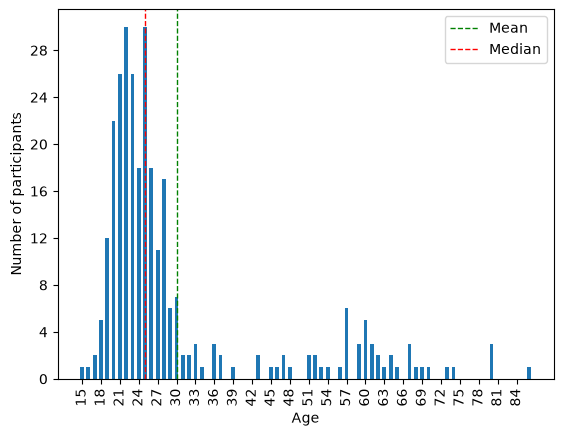
\includegraphics[width=0.85\textwidth, height=0.095\textheight, keepaspectratio]{plots/age_dist.png}
        \par\vspace{0.15em}
        {\small \textit{Figure 1: Participant age distribution ($n=295$).}}
      \end{block}

      \vspace{0.3em}

      \begin{block}{Accuracy By Musical Experience}
        \vspace{0.1em}
        \centering
        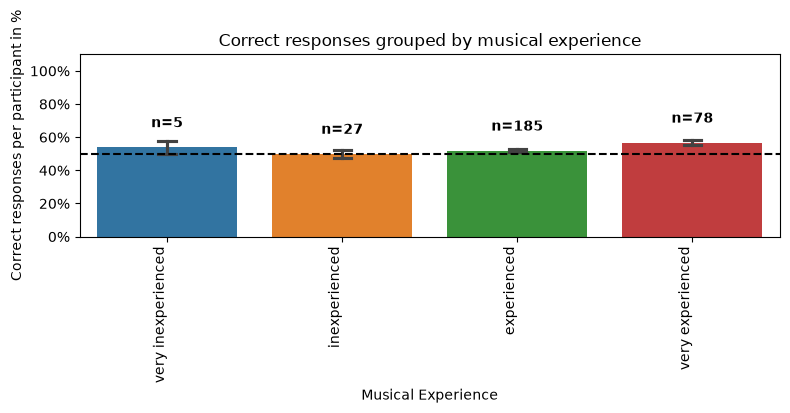
\includegraphics[width=0.85\textwidth, height=0.095\textheight, keepaspectratio]{plots/musical_exp.png}
        \par\vspace{0.15em}
        {\small \textit{Figure 2: Discrimination accuracy across participants' prior musical experience.}}
      \end{block}
    \end{column}

    \hfill

    \begin{column}{0.47\textwidth}
      \begin{block}{Choir Singers Outperform Non-Singers}
        \vspace{0.1em}
        \centering
        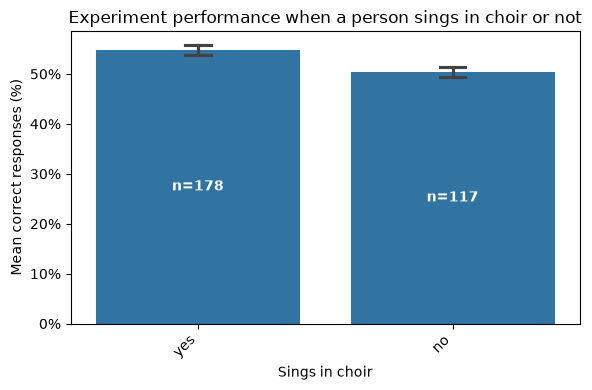
\includegraphics[width=0.85\textwidth, height=0.095\textheight, keepaspectratio]{plots/sings_in_choir.png}
        \par\vspace{0.15em}
        {\small \textit{Figure 3: Accuracy comparison by participants' choir experience.}}
      \end{block}

      \vspace{0.3em}

      \begin{block}{Trial Exposure Shifts Confidence}
        \vspace{0.1em}
        \centering
        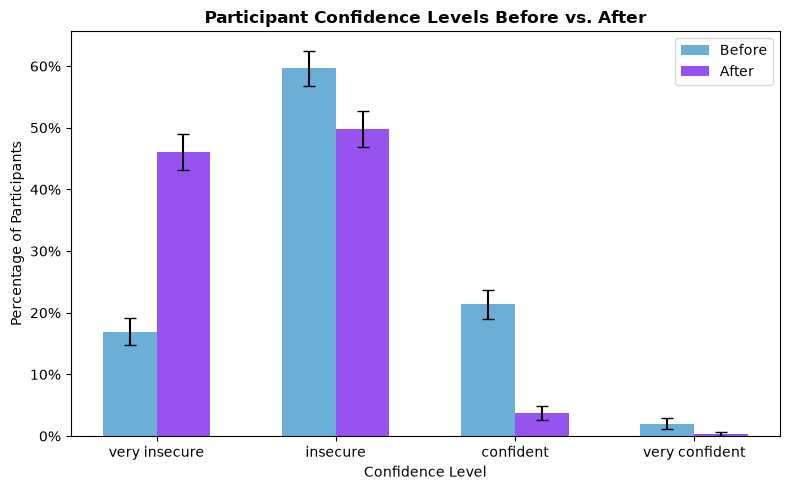
\includegraphics[width=0.89\textwidth, height=0.095\textheight, keepaspectratio]{plots/confid_before_after.png}
        \par\vspace{0.15em}
        {\small \textit{Figure 4: Self-reported confidence pre- vs.\ post-trial.}}
      \end{block}
    \end{column}
  \end{columns}

  \vspace{0.3em}

  % ==========================================
  % 3. OVERVIEW PLOT
  % ==========================================
  \begin{columns}[t]
    \begin{column}{0.47\textwidth}
      \begin{block}{Overview: Performance Per Participant}
        \vspace{0.1em}
        \centering
        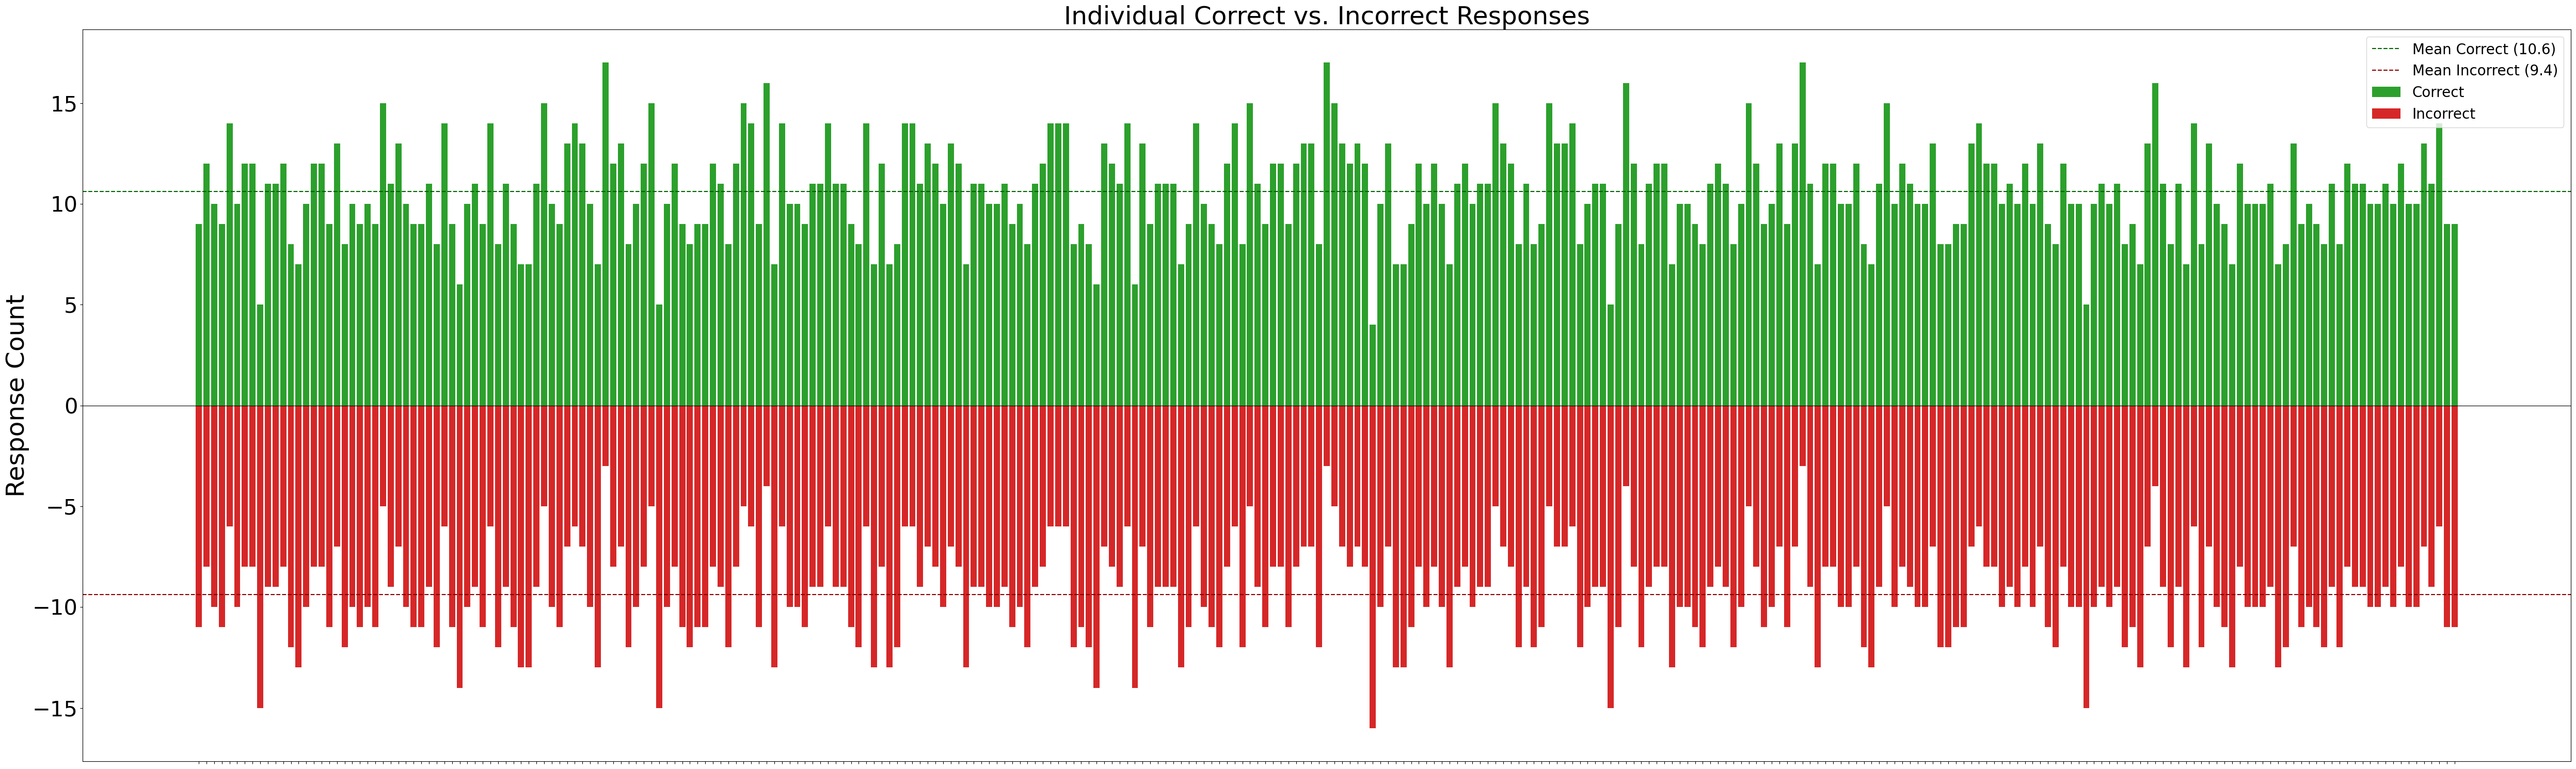
\includegraphics[width=\textwidth, height=0.10\textheight, keepaspectratio]{plots/corr_vs_incorr_indiv.png}
        \par\vspace{0.15em}
        {\small \textit{Figure 5: Individual participant accuracy scores across all trials.}}
      \end{block}
    \end{column}

    \hfill

    \begin{column}{0.47\textwidth}
      \begin{block}{Stimulus Difficulty Varies}
        \vspace{0.1em}
        \centering
        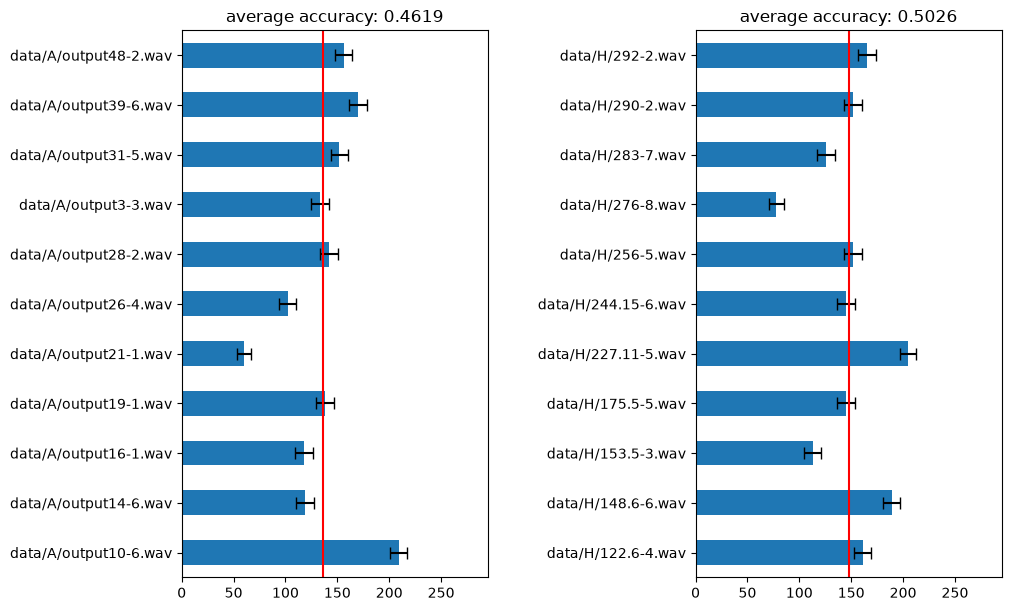
\includegraphics[width=0.85\textwidth, height=0.10\textheight, keepaspectratio]{plots/stimuli_comp.png}
        \par\vspace{0.15em}
        {\small \textit{Figure 6: Overview of individual stimulus discrimination. Left plot shows AI snippets. \\ Right plot shows human-composed snippets.}}
      \end{block}
    \end{column}
  \end{columns}

  \vspace{-0.3em}

  % ==========================================
  % 4. LIMITATIONS & FUTURE WORK
  % ==========================================
  \begin{block}{\hspace{0.5em}Limitations and Future Work}
    \vspace{-0.5em}
    \small
    \begin{columns}[t]
      \begin{column}{0.48\textwidth}
        \begin{itemize}
          \setlength\itemsep{0em}
          \item MIDI playback may lead to artifact bias.
          \item Potential selection bias in chosen stimuli.
          \item Lack of visual sheet music representation.
        \end{itemize}
      \end{column}
      \begin{column}{0.48\textwidth}
        \begin{itemize}
          \setlength\itemsep{0em}
          \item Comparison with other symbolic music generation models (AI vs. AI / AI vs. Human)
          \item Implement longer musical stimuli
          \item Expand survey towards more "artistic" musical genres
        \end{itemize}
      \end{column}
    \end{columns}
    \vspace{0.1em}
  \end{block}

  \vfill 
  \vspace{-1.8cm}
  \begin{columns}[t]

    \begin{column}{0.4\textwidth}
      \begin{block}{References}
        \vspace{0.5em}
        \printbibliography
      \end{block}
    \end{column}



% --- COLUMN 2: QR CODE & EXPERIMENT ---
    \hspace*{-0.5cm}
\begin{column}{0.4\textwidth}
  \begin{block}{Try the Experiment}
    \vspace{1em}
    \begin{minipage}[c]{0.48\textwidth}
      \centering
      \qrcode[height=5cm]{https://jasonvla.github.io/ai-chorales_website/}
    \end{minipage}%
    \hspace*{-3cm}
    \begin{minipage}[c]{0.48\textwidth}
      \centering
      \textbf{Can you distinguish AI from human-composed?}\\[-0.2em]
      $\leftarrow$ Scan to test your skills\\[-0.2em]
      \href{https://jasonvla.github.io/ai-chorales_website/}{\texttt{\small jasonvla.github.io/ai-chorales\_website}}
    \end{minipage}
    \vspace{0.1em}
  \end{block}
\end{column}

    \hfill

    % --- COLUMN 3: INSTITUTIONAL LOGO ---
    \begin{column}{0.1\textwidth}
    \vspace{4.5em}
    \hspace*{0.1em}
      \centering
      
\includegraphics[width=\linewidth, keepaspectratio]{unilogo_Vektor_CMYK-eps-converted-to.pdf}
    \end{column}
  \end{columns}
\end{frame}

\end{document}